\documentclass[12pt]{article}
\usepackage{amsmath}
\usepackage{graphicx}
\usepackage{enumerate}
\usepackage{natbib}
\usepackage{url} % not crucial - just used below for the URL 

%\pdfminorversion=4
% NOTE: To produce blinded version, replace "0" with "1" below.
\newcommand{\blind}{1}
\newcommand{\fulltitle}{Estimating the duration of positivity for SARS-CoV-2 from doubly interval censored data with missed infections}

% DON'T change margins - should be 1 inch all around.
\addtolength{\oddsidemargin}{-.5in}%
\addtolength{\evensidemargin}{-1in}%
\addtolength{\textwidth}{1in}%
\addtolength{\textheight}{1.7in}%
\addtolength{\topmargin}{-1in}%

%% ABOVE THIS LINE IS JASA TEMPLATE
%% BELOW THIS LINE IS MY STUFF

\usepackage[utf8]{inputenc}
\usepackage{amssymb}
\usepackage{floatpag}
\usepackage{bm}
% \usepackage{algorithm2e}
\usepackage[unicode,psdextra]{hyperref}
\usepackage[nameinlink]{cleveref}
\usepackage{csquotes}
\usepackage[T1]{fontenc}
\usepackage{textcomp} % provide symbols
\usepackage{xr}
\usepackage{afterpage}
\usepackage{caption}
\usepackage{numprint}
\npfourdigitnosep
\npdecimalsign{.}
% \usepackage{microtype}
\usepackage{todonotes}

% Generic maths commands
\def\reals{\mathbb{R}}
\def\nats{\mathbb{N}}
\def\sampSpace{\mathcal{X}}
\def\dist{\sim}
\DeclareMathOperator{\E}{\mathbb{E}}
\DeclareMathOperator{\V}{\mathbb{V}}
\DeclareMathOperator{\I}{\mathbb{I}}
\DeclareMathOperator{\prob}{\mathbb{P}}
\DeclareMathOperator{\p}{\pi}
\DeclareMathOperator{\var}{\mathbb{V}}
\DeclareMathOperator{\indicator}{\mathbb{I}}
\DeclareMathOperator{\cov}{Cov}
\DeclareMathOperator{\cor}{Cor}
\DeclareMathOperator{\logit}{logit}
\DeclareMathOperator{\Ber}{Bernoulli}
\DeclareMathOperator{\Bin}{Binomial}
\DeclareMathOperator{\Poi}{Poisson}
\DeclareMathOperator{\BetaDist}{Beta}
\DeclareMathOperator{\Exponential}{Exponential}
\DeclareMathOperator{\NBr}{NegBin}
\newcommand{\NBc}{\NBr_{c}}
\newcommand{\NBs}{\NBr_{s}}
\DeclareMathOperator{\BB}{BetaBin}
\DeclareMathOperator{\GamDist}{Gamma}
\DeclareMathOperator{\MN}{Multinomial}
\DeclareMathOperator{\N}{N}
\DeclareMathOperator{\MNorm}{N}
\DeclareMathOperator{\LN}{LN}
\DeclareMathOperator{\LKJ}{LKJ}
\DeclareMathOperator{\expit}{expit}
\newcommand\matr{\bm}
\newcommand\set{\mathcal}
\renewcommand{\vec}[1]{\bm{#1}}
\newcommand{\ssep}{:}
\DeclareMathOperator*{\argmax}{arg\,max}

% Thesis-specific maths commands
\newcommand{\dmax}{d_\text{max}}
\newcommand{\psens}{p_\text{sens}}
\newcommand{\psenss}{p_\text{sens}^{(s)}}
\newcommand{\psensi}{p_\text{sens}^{(i)}}
\newcommand{\ntot}{n_\text{tot}}
\newcommand{\ndet}{n_\text{d}}
\newcommand{\nnodet}{n_\text{u}}
\newcommand{\pnodet}{p_\text{u}}
\newcommand{\Npop}{N_\text{pop}}
\newcommand{\Ncis}{N_\text{CIS}}
\newcommand{\ncis}{\vec{n_\text{CIS}}}
\newcommand{\na}{\vec{n}_\text{obs}}
\newcommand{\pcis}{\vec{p_\text{CIS}}}
\newcommand{\sched}{\mathbb{T}}
\newcommand{\nsched}{n_{\sched}}
\newcommand{\inform}{{_{\text{inform}}}}


%% Bibliography
% \usepackage[authordate-trad,backend=biber]{biblatex-chicago}
% \addbibresource{references.bib}

% Macros for common abbreviations to get the spacing right
% See: https://stackoverflow.com/questions/3282319/correct-way-to-define-macros-etc-ie-in-latex
\usepackage{xspace}
\makeatletter
\DeclareRobustCommand\onedot{\futurelet\@let@token\@onedot}
\def\@onedot{\ifx\@let@token.\else.\null\fi\xspace}
\def\eg{e.g\onedot} \def\Eg{{E.g}\onedot}
\def\ie{i.e\onedot} \def\Ie{{I.e}\onedot}
\def\cf{c.f\onedot} \def\Cf{{C.f}\onedot}
\def\etc{etc\onedot} \def\vs{{vs}\onedot}
\def\wrt{w.r.t\onedot} \def\dof{d.o.f\onedot}
\def\etal{et al\onedot}
\makeatother

%% LINE NUMBERS
% \usepackage{lineno} % Include the package for line numbering
% \linenumbers % Activates line numbering for the document

\begin{document}

%\bibliographystyle{natbib}

\def\spacingset#1{\renewcommand{\baselinestretch}%
{#1}\small\normalsize} \spacingset{1}


%%%%%%%%%%%%%%%%%%%%%%%%%%%%%%%%%%%%%%%%%%%%%%%%%%%%%%%%%%%%%%%%%%%%%%%%%%%%%%

\if1\blind
{
  \title{\bf \fulltitle}
  \author{%
    Blake, TBC, Birrell, De Angelis  
    % Author 1\thanks{
    % The authors gratefully acknowledge \textit{please remember to list all relevant funding sources in the unblinded version}}\hspace{.2cm}\\
    % Department of YYY, University of XXX\\
    % and \\
    % Author 2 \\
    % Department of ZZZ, University of WWW}
  }
  \maketitle
} \fi

\if0\blind
{
  \bigskip
  \bigskip
  \bigskip
  \begin{center}
    {\LARGE\bf \fulltitle}
\end{center}
  \medskip
} \fi

\bigskip
\begin{abstract}
The text of your abstract. 200 or fewer words.
\end{abstract}

\noindent%
{\it Keywords:}  3 to 6 keywords, that do not appear in the title
\vfill

\newpage

\textbf{Notes / thoughts on current version}
\begin{itemize}
    \item Some of the derivations can be moved to a supplement (cut 2--3 pages).
    \item Need to rearranage the ATACCC stuff --- add some details of what I did (thesis ch 4) and move stuff from prior info section into supplement.
    \item Probably don't need some of the figures (maybe 5--8)?
    \item Should the sensitivity analyses (figs 13/14 be in the main text)?
    \item The above changes make this about the right length.
\end{itemize}

The \textbf{format requirements from JASA} are at \url{https://www.tandfonline.com/journals/uasa20}.
\begin{itemize}
    \item Should be written with the following elements in the following order: title page; author footnote; abstract; keywords; article text (table(s); figures); acknowledgments; appendices; references
    \item Should be no more than 35 pages, including the abstract, figures, tables, and references. Appendices, proofs, and other supporting material should be placed in a separate supplement file (anonymized for review)
    \item Should contain an unstructured abstract of 200 words.
    \item Should contain between 3 and 5 keywords. Read making your article more discoverable, including information on choosing a title and search engine optimization.
    \item JASA requires that all papers be formatted for 8 1/2 x 11-inch paper, one side only.
    \item 12 point, double-spaced font (which we define as 26 lines of text per page)
    \item the average JASA paper is about 30 manuscript pages (with the above page format and including all appendices, references, tables, and figures), and it is very uncommon for papers much longer than about 35 pages to appear in JASA. 
\end{itemize}

\newpage
\spacingset{1.9} % DON'T change the spacing!
\section{Introduction}
\label{sec:intro}


\section{Problem description}

The CIS~\citep{CIS} was setup in April 2020.
The dataset is globally unique in providing a representative, longitudinal, and large-scale study across the pandemic.
% Initially, it was limited to England, but expanded to cover the whole of the UK in September 2020.
Enrolment was continuous until 31st Jan 2022, with data collected until 13th Mar 2023~\citep{weiRisk}. 

The CIS had a household-based design inviting all individuals aged 2 and over from selected households.
Once invited, an enrolment swab would be taken at the first visit followed by 4 further weekly visits (giving a total of 5 swabs on days 0, 7, 14, 21, 28 relative to enrolment) after which visits were monthly.
Swabs were tested for the presence of SARS-CoV-2 using RT-PCR.
In reality, visits were often not on this precise schedule, and occasionally missed.
A full description of the study can be found in the study protocol~\citep{cisProtocol}.

Positive tests are grouped into \emph{infection episodes} which are assumed to originate from the same infection (using the procedure described in \citep{weiRisk}).
The crucial features of an infection episode are the start and end times of the infection.
Ignoring misclassified test results, latent start time of infection episode $j$, $B_j$, can be bounded as between the day after the last negative test, $l_j^{(b)}$, and the day of the first positive test, $r_j^{(b)}$.
Similarly, the latent end time of infection episode $i$, $E_j$, can be bounded as between the day of the last positive test, $l_j^{(e)}$, and the day before the following negative test, $r_j^{(e)}$.

\todo[inline]{Include here definitions of the key quantities of interest: the duration of an episode, the beginning and end of an episode, and the survival function.}

For privacy reasons, the CIS data are stored in the ONS's SRS (Secure Research Service).
The SRS is a Trusted Research Environment (TRE) that allows researchers to access sensitive data in a secure environment.
The SRS must be used to perform analyses using individual-level data.
Therefore, computationally efficient approaches must be taken to this work.

\subsection{Undetected infections}

\subsection{Double interval censoring} \label{perf-test:sec:interval-censoring}

\subsection{False negatives}

\section{Methodology}

\subsection{Survival analysis framework}

We start by developing a computationally feasible Bayesian statistical model accounting for double interval censoring and undetected episodes, assuming that there are no misclassified test results.

We analyse the $\ndet = \numprint{4800}$ episodes with their first positive test between 10 Oct 2020 and 6 Dec 2020 inclusive, with negatives bounding the start and end time of the episode; we refer to these episodes as \emph{detected}; in \cref{perf-test:sec:prob-undetected} we formalise the conditions for an episode to be detected.
Days in this period are denoted as $t = 1, \dots, T$.
Only the first positive test in the episode needs to occur in $[1, T]$, the remaining tests can occur outside this period.
We use these episodes because a negative test before the start of the episode provides a lower bound on the episode's start time; otherwise, there is little information on its length.
For a small number\todo{how many?} number of episodes, the individual is lost to follow-up before they test negative; these episodes are excluded from the analysis.

These episodes occur within the cohort of $\Ncis = \numprint{437590}$ individuals who could have had a detected episode.
This is all individuals enrolled in CIS with at least one test in the interval $[1, T]$.

An individual $i$ has a \emph{test schedule} $\sched_i$.
The test schedule $\sched_i$ is the set of times at which individual $i$ is tested, starting from their last test prior to time 1, if it exists, or their time of enrolment otherwise; note that $\sched_i$ includes any tests that occur after $T$.
For example, for the individual in \cref{perf-test:fig:double-interval-censor}, $\sched_i = \{ 0, 7, 14, 21, 28, 56 \}$.
Each individual has exactly one test schedule, but it is possible that $\sched_i = \sched_{i'}$ for $i \neq i'$.
We assume that the test schedules are uninformative on all quantities of interest because they are part of the study design, and all probabilities are implicitly conditioned on them.

The relevant observations for a detected episode $j$ are $o_j = [l_j^{(b)}, r_j^{(b)}, l_j^{(e)}, r_j^{(e)}, i_j]^T$ where $i_j$ is the individual episode $j$ occurred in and the other variables are defined as in \cref{sec:problem-description}.
When assuming all tests are correctly classified, $l_j^{(b)}$ is the day after the last negative test before the episode, $r_j^{(b)}$ is the day of the first positive test, $l_j^{(e)}$ is the day of the last positive test, and $r_j^{(e)}$ is the day before the first negative test after the episode.
In this case, $o_j$ is fully determined by $\sched_{i_j}$, $b_j$, and $e_j$.

In addition, $\nnodet$ undetected episodes occurred; $\nnodet$ is latent.
If $j$ is undetected, then define $o_j = \emptyset$.

The total number of infection episodes in the cohort is $\ntot = \ndet + \nnodet$ and we index them with $j = 1, \dots, \ntot$.

\subsubsection{Posterior density}

The target of inference is $\vec{\theta}$, the parameters of the survival function $S_{\vec{\theta}}(t) = \prob(D_j \geq t \mid \vec\theta)$; its composition is discussed in \cref{sec:parameters-priors}.

The observation $o_j$ is a realisation of the discrete random variable $O_j$.
Define $O_j$'s state space as $\set{E}' = \{ \emptyset \} \cup \set{E}$ where $\set{E} = \{ \vec{\nu}_1, \dots, \vec{\nu}_{N_E} \}$ is the set of all $N_E$ (a priori) possible unique observations of detected episodes.
Therefore, $\vec{\nu}_k = [l^{(b)}_k, r^{(b)}_k, l^{(e)}_k, r^{(e)}_k, i_k]^T$ for $k = 1, \dots, N_E$.

Let $p_k = \prob(O_j = \vec{\nu}_k \mid \vec{\theta})$, the probability that $O_j$ takes the value $\vec{\nu}_k$.
Similarly, let $p_u = \prob(O_j = \emptyset \mid \vec{\theta})$, the probability that $j$ is undetected.
Then, the probability distribution for $O_j$ is specified by $\vec{p} = [p_1, \dots, p_{N_E}, p_u]^T$.

Let $n_k$ denote the number of times $\vec{\nu}_k$ is observed; $\nnodet$ denote the latent number of undetected episodes; and $\vec{n} = [n_1, \dots, n_{N_E}, \nnodet]^T$.
Formally, $n_k = \sum_{j=1}^{\ntot} \indicator(O_j = \vec{\nu}_k)$ and $\nnodet = \sum_{j=1}^{\ntot} \indicator(O_j = \emptyset)$.
Hence, $\ndet = \sum_{k=1}^{N_E} n_k$.
Assume, for tractability, that the events $O_j = \vec{\nu}_k$ and $O_{j'} = \vec{\nu}_{k'}$ are independent for $j \neq j'$ (conditional on $\theta$); this assumption is discussed in \cref{sec:discussion}.
Hence:
\begin{align}
  \vec{n} \mid \ntot, \vec{\theta} &\dist \MN(\ntot, \vec{p})
\intertext{that is:}
  p(\vec{n} \mid \ntot, \vec{\theta}) &= \frac{\ntot!}{\nnodet!\prod_{k=1}^{N_D} n_k!} p_u^{\nnodet} \prod_{k=1}^{N_D} p_k^{n_k}.
  \label{perf-test:eq:multinomial-ll}
\end{align}
\begin{figure}
\makebox[\textwidth][c]{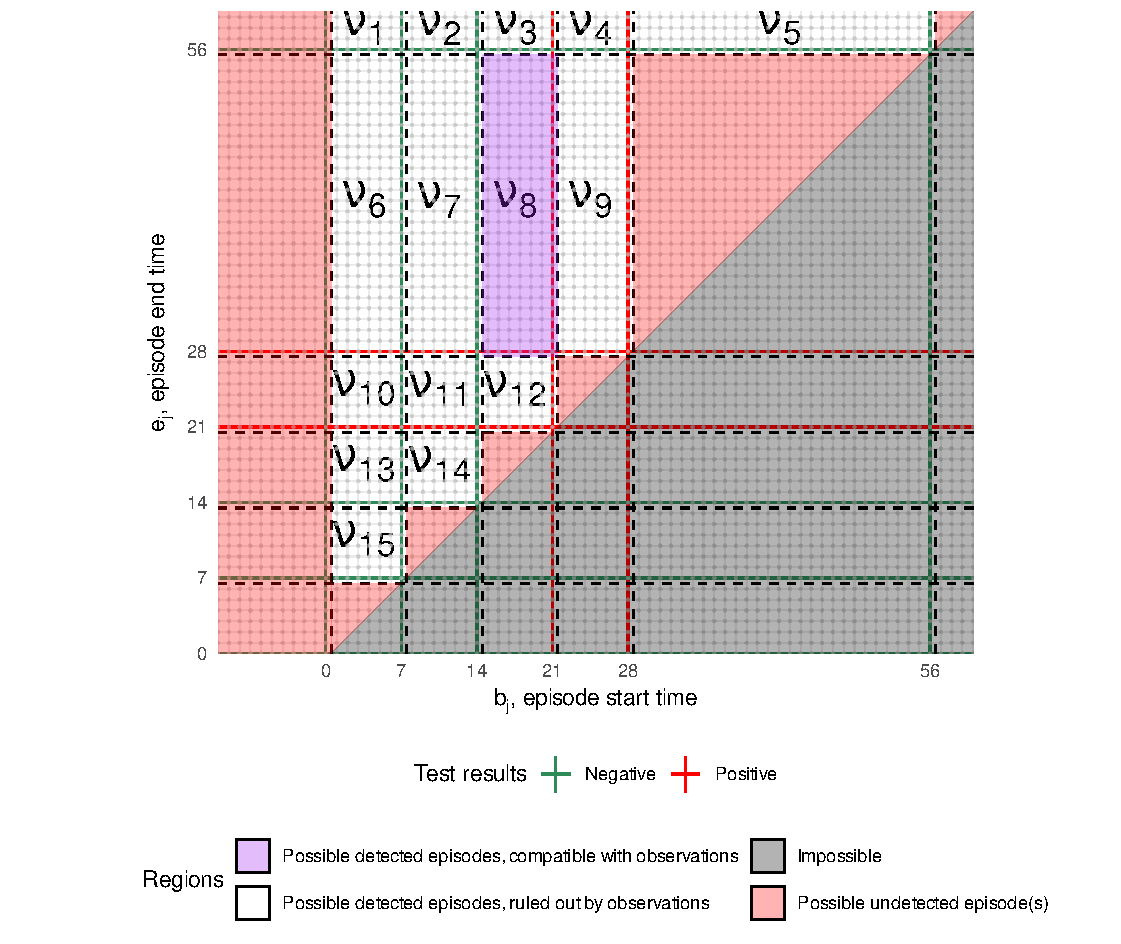
\includegraphics[width=0.9\paperwidth]{figures/output/regions_diag}}
\thisfloatpagestyle{empty}
\caption[Episode regions]{%
  Each dot is a combination of $b_j$ and $e_j$ for an arbitrary individual $i$.
  Each box, bounded by dashed lines, are combinations giving $O_j = \vec{\nu}_k$, $k$ corresponding to the numeric label; labels are arbitrary but unique across all individuals.
  $i$ had negative tests at times 0, 7, 14, 56, and 84 (not shown) and positive tests at times 21 and 28.
  The purple region corresponds to the doubly interval censored episode in this individual.
  That is, $n_8 = 1$ and $n_k = 0$ for $k = 1, \dots, 7, 9, \dots, 15$.
  The red region corresponds to combinations giving $O_j = \emptyset$.
  Impossible region violates $b_j \leq e_j$.
}
\label{perf-test:fig:partitionSpace}
\end{figure}

In the CIS data, each $n_k$ ($k \neq u$) is observed as either 0 or 1.
Define $\set{D} = \{ k \ssep n_k = 1 \}$, the detected episodes.
Furthermore, note that the support of the multinomial distribution requires that $\nnodet = \ntot - \ndet$.
Let $\na = [n_{1}, \dots, n_{N_E}]^T$ be the observed portion of $\vec{n}$.
Then \cref{perf-test:eq:multinomial-ll} simplifies to:
\begin{align}
  p(\vec{n} \mid \ntot, \vec{\theta})
  &= p(\na \mid \ntot, \vec{\theta}) \\
  &= \frac{\ntot!}{(\ntot - \ndet)!} p_u^{\ntot-\ndet} \prod_{k \in \set{D}} p_k.
  \label{perf-test:eq:multinomial}
\end{align}

The relevant information from the CIS data is fully contained in the vector $\na$.
Therefore, the posterior of interest is (see\todo{ref appendix} for the full derivation):
\begin{align}
p(\vec{\theta} \mid \na)
&\propto  p(\vec{\theta}) \left( \prod_{k \in \set{D}} p_k \right) \left( \sum_{\ntot=\ndet}^\infty p(\ntot \mid \vec{\theta}) \frac{\ntot!}{(\ntot - \ndet)!} \pnodet^{\ntot - \ndet} \right).
\label{perf-test:eq:posterior1}
\end{align}

For mathematical convenience, we assume the prior $\ntot \dist \NBc(\mu, r)$, and that it is independent of $\vec{\theta}$, the parameters of the survival distribution.
In this case \cref{perf-test:eq:posterior1} simplifies to (see\todo{cite appropriate appendix}):
\begin{align}
p(\vec{\theta} \mid \na)
&\propto p(\vec{\theta}) \left( \prod_{i \in \set{D}} p_k \right) (r + \mu (1- \pnodet))^{-(r+\ndet)} \label{perf-test:eq:full-posterior}.
\end{align}

The rest of this section derives expressions for each of $p_{k}$, $p_{u}$ and $\eta$.

Decompose $p_k$ as $p_k = p_{ik} \prob(i_j = i_k \mid \vec{\theta})$
where $p_{ik} = \prob(O_j = \vec{\nu}_k \mid i_j = i_k, \vec{\theta})$.
% This is valid as $\prob(O_j = \nu_k \mid i_j \neq i_k) = 0$ due to the condition here being equivalent to equating the two vectors' final elements.
Assume that each infection episode occurs independently and with equal probability in any individual, \ie $\prob(i_j = i_k) = 1/\Ncis$ for all $j$ and $k$, and $B_j$ takes values with uniform probability from its state space.

Therefore, $p_{ik}$ takes the standard form of the likelihood for doubly interval censored data without truncation (see\todo{ref appendix} for details):
\begin{align}
p_{ik}
\propto& \sum_{b = l_k^{(b)}}^{r_k^{(b)}} \left( S_{\vec{\theta}}(l_k^{(e)} - b + 1) - S_{\vec{\theta}}(r_k^{(e)} - b + 2) \right).
\label{perf-test:eq:pia}
\end{align}

The remaining component of \cref{perf-test:eq:full-posterior} required is $1- p_u$, one minus the probability of missing an infection, \ie the probability of detecting an infection.

\subsubsection{Deriving $1 - p_u$} \label{perf-test:sec:prob-undetected}

The final component of \cref{perf-test:eq:full-posterior} required is $1 - p_u$.
Recall the definition $p_u = \prob(O_j = \emptyset \mid \vec{\theta})$.
Therefore:
\begin{align}
  1 - p_u
  &= 1 - \sum_{i=1}^{\Ncis} \prob(O_j = \emptyset, i_j = i \mid \vec{\theta}) \\
  &= 1 - \sum_{i=1}^{\Ncis} \prob(O_j = \emptyset \mid i_j = i, \vec{\theta}) P(i_j = i \mid \vec{\theta}) \\
  &= 1 - \frac{1}{\Ncis}\sum_{i=1}^{\Ncis} \prob(O_j = \emptyset \mid i_j = i, \vec{\theta}) \\
  &= \frac{1}{\Ncis} \sum_{i=1}^{\Ncis} (1 - \prob(O_j = \emptyset \mid i_j = i, \vec{\theta}))
  \label{perf-test:eq:pu}
\end{align}
assuming $P(i_j = i \mid \vec{\theta}) = 1/\Ncis$ as before.
Let $p_{iu} = \prob(O_j = \emptyset \mid i_j = i, \vec{\theta})$.
Therefore, the crucial component is $1 - p_{iu}$.
This is one minus the probability that an episode in individual $i$ was undetected, \ie the probability of the episode being detected.

An episode $j$ in individual $i_j$ is detected if and only if all the following conditions are met.
\begin{enumerate}
    \item $\exists t \in \sched_{i_j}$ such that $b_j \leq t \leq e_j$; this condition is equivalent to having at least one positive test for the episode.
    \item $b_j > \min \sched_{i_j}$.
      For individuals enrolled during the period considered ($\min \sched_{i_j} > 0$), this ensures that the beginning of the episode is lower bounded; thereby adjusting for those who enrolled during the period being less likely to have a detected infection.
      For individuals enrolled prior to the period considered ($\min \sched_{i_j} \leq 0$), this means that the episode was not detected prior to time 1.
    \item $b_j \leq T_{i_j}$ where $T_{i_j} = \max \{ t \in \sched_{i_j} \ssep t \leq T \}$ is the last time that $i_j$ is tested in the period, meaning that the test is detected within the period.
    \item $\exists t \in \sched_{i_j}$ such that $t > e_j$, upper bounding the end of the episode.
      For episodes detected in the period we consider, a negligible number of episodes are excluded due to this critera.
      It only occurs in individuals lost to follow-up; therefore, we neglect this possibility.
      % For a new context, including recent infections, this condition could be relaxed by considering episodes that do not meet this criterion as right censored.
\end{enumerate}

% An episode is undetected if and only if no tests are performed during the episode or if there was no negative test prior to the episode.
% Equivalently, that the first test at or after $b$ is after $e$, or that there is no negative test prior to $b$.
First define $\tau_{\sched_i}(t)$ as the time until the next test at or after time $t$ in the schedule $\sched_i$:
\begin{align}
\tau_{\sched_i}(t) &= \min \{ t' \in \sched_i : t' \geq t \} - t
\label{perf-test:eq:tau-def}
\end{align}
% defining $\min \emptyset = \infty$; \ie $\tau_{\sched_i}(t) = \infty$ if there is no $t' \in \sched_i$ such that $t' \geq t$.
The first condition can now be expressed as $e_j \geq b_j + \tau_{\sched_{i_j}}(b_j)$.
Equivalently, $d_j \geq \tau_{\sched_{i_j}}(b_j) + 1$.
% The fourth condition can be expressed as $\tau_{\sched_{i_j}}(b_j) < \infty$.


% Then $\Omega_i$ can be written as:
% \begin{align}
% \Omega_i = \{ (b, e) \ssep \tau_{\sched_i}(b) + b > e \vee b \leq \min(\sched_i) \}.
% \end{align}
Therefore, omitting the conditioning on $\vec{\theta}$ and $i_j = i$:
\begin{align}
1 - p_{iu}
% &= 1 - \prob((B_{j}, E_{j}) \in \Omega_i) \\
&= \prob(D_j \geq \tau_{\sched_{i}}(B_j)+ 1, \min \sched_{i_j} < B_j \leq T_{i_j}) \\
&= \sum_{b = \min \sched_{i} + 1}^{T_{i_j}} \prob(D_j \geq \tau_{\sched_{i}}(b) + 1 \mid B_j = b) \prob(B_j = b)\\
&\propto \sum_{b = \min \sched_{i} + 1}^{T_{i_j}} S_{\vec{\theta}}(\tau_{\sched_{i}}(b) + 1).
\label{perf-test:eq:piu}
\end{align}

Substituting into \cref{perf-test:eq:pu}:
\begin{align}
1 - p_u
& \propto \sum_{i=1}^{\Ncis} \sum_{b = \min \sched_{i} + 1}^{T_{i_j}} S_{\vec{\theta}}(\tau_{\sched_{i}}(b) + 1).
\end{align}

\subsection{False negatives}

Now we modify the survival framework to incorporate false negatives (\ie allowing $\psens < 1$).
Using a simple model, in particular a constant test sensitivity, means calculating the likelihood remains tractable.

We start, in \cref{imperf-test:sec:notation}, by introducing some additional notation needed.
We then modify the components of the likelihood in \cref{imperf-test:sec:modifying-p_ia,imperf-test:sec:modifying-p_iu} to incorporate false negatives.


\subsubsection{Notation} \label{imperf-test:sec:notation}

Introducing false negatives means that $O_j$, the observation vector of episode $j$, is now random, even if $B_j$ and $E_j$ are known.
Therefore, the results between the tests that bound episode $j$'s beginning and end times should now enter into the likelihood.
For tractability, we include only tests between the negative tests at $l_j^{(b)}-1$ and $r_j^{(e)}+1$. 

To formalise this, we define analogous variables to those in \cref{E-perf-test:sec:posterior}.
To start with, define the relevant testing times for any episode $j$ with $O_j = \vec{\nu}_k$ as $\sched'_k = \{ t \in \sched_{i_k} \ssep r_k^{(b)} \leq t \leq r_k^{(e)} + 1 \}$ and let $m_k$ denote the size of this set.
Denote the elements of $\sched'_k$ by $t_{k,1} < \dots < t_{k,m_k}$.
Let $\set{E}' = \{ \vec{\nu}_1', \dots, \vec{\nu}_{N_E'}' \}$ be a new set of possible observations of detected episodes, including the pattern of positive and negative tests.
Represent the observations such that for any $\vec{\nu}_k' \in \set{E}'$, $\vec{\nu}_k' = [\vec{\nu}_{k}, \vec{y}_k]^T$, where $\vec{y}_k \in \{ 0, 1 \}^{m_k}$ with $y_{k,l}$ being the test result at time $t_{k,l}$.

$\vec{\nu}'_k \in \set{E}'$ occurs if and only if all the following conditions are met.
\begin{enumerate}
  \item $\vec{\nu}_k \in \set{E}$.
  \item The elements of $\vec{y}_k$ corresponding to the tests at times $r_k^{(b)}$ and $l_k^{(e)}$ are positive, \ie $y_{k,1} = y_{k,m_k-1} = 1$.
  \item The element of $\vec{y}_k$ corresponding to the test at time $r_k^{(e)} + 1$ is negative, \ie $y_{k,m_k} = 0$.
\end{enumerate}
The final two conditions are due to the construction of the intervals as positive and negative tests bounding the beginning and end times of the episode.
As condition 2 requires $y_{k,1} = 1$ and condition 3 requires $y_{k,m_k} = 0$, these conditions can only occur if $m_k \neq 0$.
Therefore, $m_k \geq 2$.

Let $O'(j)$ be the observations generated by episode $j$ including the new vector of results.
As before, $O'(j) \in \set{E}'$ indicates that episode $j$ was detected; otherwise, $O'(j) = \emptyset$.

Similarly, we define $p_k'$, $p_{ik}'$, $p_u'$, and $p_{iu}'$ to replace $p_k'$, $p_{ik}'$, $p_u'$, and $p_{iu}'$ respectively.
\begin{align}
    p_{ik}' &= \prob(O'(j) = \vec{\nu}'_k \mid i_j = i_k, \vec{\theta}) \\
    p_k' &= \frac{1}{\Ncis} p_{ik}' \\
    p_{iu}' &= \prob(O'(j) = \emptyset \mid i_j = i_k, \vec{\theta}) \\
    p_u' &= \frac{1}{\Ncis} \sum_{i=1}^{\Ncis} p_{iu}'.
\end{align}

\subsubsection{Deriving $p'_{ik}$} \label{imperf-test:sec:modifying-p_ia}

We will modify $p_{ik}$ to form $p_{ik}' = \prob(O'(j) = \vec{\nu}'_k \mid i_j = i_k, \vec{\theta})$, taking into account false negatives.
We consider a mixture of two scenarios, whether the final test in $\sched'_{k}$ is a false negative, with the mixture probability determined by the test sensitivity.

Similar likelihoods have previously appeared in the literature~\citep[e.g.][eq.\ (2)]{piresIntervalMisclassify}.
However, this prior work was for singly interval censored data; incorporating the double interval censored nature of the CIS data involves summing over the possible episode start times.

% We proceed by assuming that we have observed an arbitrary episode:
% \begin{align}
%   O'(j) = [[l_k^{(b)}, r_k^{(b)}, l_k^{(e)}, r_k^{(e)}, i_j]^T, \vec{y}_k]^T.
% \end{align}
% We derive $p_k$ by considering the generating process that could have produced this episode.

For tractability, assume that the negative test bounding the start of the episode, on day $l_k^{(b)}-1$, is a true negative.
This assumption is reasonable because, since a positive test follows at $r_k^{(b)}$, the negative at $l_k^{(b)}-1$ is likely early in the infection and the test sensitivity is high early in an infection.
True negatives occur with probability 1, and hence this test does not contribute to the likelihood.

As we assume that there are no false positives, the infection episode must span at least the period $[r^{(b)}_k, l^{(e)}_k]$, a period starting and ending with a positive test.
This includes all $t \in \sched'_k$ except $t = r_k^{(e)}+1$.
Therefore, the test results $\vec{y}_k$, except the test at $r_k^{(e)}+1$, are either true positives or false negatives.
This gives $t_+ = \sum_{l=1}^{m_k-1} y_{k,l}(t)$ true positives and $f_- = \sum_{l=1}^{m_k-1} (1 - y_{k,l}(t))$ false negatives.

Consider the negative test at $r_k^{(e)}+1$, the first negative after the start of the episode which may be a false negative.
It is a false negative if and only if the episode ends at or after the test, \ie $E_j > r_k^{(e)}$.
We proceed by first considering whether this is the case and conditioning on $B_j = b$.
Then, we combine the cases and remove the conditioning.

First, the case when $E_j \leq r_k^{(e)}$.
In this case, the test at $r_k^{(e)}+1$ is a true negative and the end of the episode is interval censored as in the previous chapter.
% In this case, the test at $r_k^{(e)} + 1$ is a true negative, as are all other tests not in $\sched'_{k}$.
The true negative occurs with probability 1, by the assumption of no false positives.
\begin{align}
&\prob(O'(j) = \vec{\nu}_k', E_j \leq r_k^{(e)} \mid B_j = b, i_j = i_k, \psens, \vec{\theta}) \\
&= \prob(O'(j) = \vec{\nu}_k', l_k^{(e)} \leq E_j \leq r_k^{(e)} \mid B_j = b, i_j = i_k, \psens, \vec{\theta}) &\text{the test at $l_k^{(e)}$ is positive} \\
&= \prob(O'(j) = \vec{\nu}_k' \mid l_k^{(e)} \leq E_j \leq r_k^{(e)}, B_j = b, i_j = i_k, \psens, \vec{\theta}) \\
&\ \ \  \times \prob(l_k^{(e)} \leq E_j \leq r_k^{(e)} \mid B_j = b, i_j = i_k, \psens, \vec{\theta}) \\
&= p_\text{sens}^{t_+} (1 - p_\text{sens})^{f_-} \left( S_{\vec{\theta}}(l_k^{(e)} - b + 1) - S_{\vec{\theta}}(r_k^{(e)} - b + 2) \right)
\label{imperf-test:eq:ll-ei-lt-ri}
\end{align}

Second, the case when $E_j > r_k^{(e)}$.
In this case, the test at $r_k^{(e)}+1$ is a false negative, occurring with probability $(1 - p_\text{sens})$.
To avoid having to consider tests after $r_k^{(e)}$, which could greatly complicate the likelihood, we model this case as the episode being right censored at $r_k^{(e)}$.
Taking the same approach as before:
\begin{align}
&\prob(O'(j) = \vec{\nu}_k', E_j > r_k^{(e)} \mid B_j = b, i_j = i_k, \psens, \vec{\theta}) \\
&= \prob(O'(j) = \vec{\nu}_k' \mid E_j > r_k^{(e)}, B_j = b, i_j = i_k, \psens, \vec{\theta}) \\
  &\ \ \  \times \prob(E_j > r_k^{(e)} \mid B_j = b, i_j = i_k, \psens, \vec{\theta}) \\
&= p_\text{sens}^{t_+} (1 - p_\text{sens})^{f_-} (1 - p_\text{sens}) S_{\vec{\theta}}(r_k^{(e)} - b + 2)
\label{imperf-test:eq:ll-ei-gt-ri}
\end{align}

These expressions can now be used to derive $p'_{ik}$.
First, augment the data with $b$, and split into the cases just discussed, omitting the conditioning on $\psens$, $\vec{\theta}$, and $i_j = i_k$:
\begin{align}
p_{ik}'
=& \prob(O'(j) = \vec{\nu}_k') \\
=& \sum_{b = l_k^{(b)}}^{r_k^{(b)}} \left( \prob(O'(j) = \vec{\nu}_k', E_j \leq r_k^{(e)} \mid B_j = b) + \prob(O'(j) = \vec{\nu}_k, E_j > r_k^{(e)} \mid B_j = b) \right) \prob(B_j = b). \\
\intertext{Now, substitute in \cref{imperf-test:eq:ll-ei-lt-ri,imperf-test:eq:ll-ei-gt-ri} and take out the common factor:}
=\ &  p_\text{sens}^{t_+} (1 - p_\text{sens})^{f_-} \\
 & \times \sum_{b = l_k^{(b)}}^{r_k^{(b)}} \left( S_{\vec{\theta}}(l_k^{(e)} - b + 1) - S_{\vec{\theta}}(r_k^{(e)} - b + 2) + (1 - p_\text{sens}) S_{\vec{\theta}}(r_k^{(e)} - b + 2) \right) \\ 
  & \times \prob(B_j = b \mid p_\text{sens}, \vec{\theta}) \\
=\ &  p_\text{sens}^{t_+} (1 - p_\text{sens})^{f_-} \\
  & \times \sum_{b = l_k^{(b)}}^{r_k^{(b)}} \left( S_{\vec{\theta}}(l_k^{(e)} - b + 1) - p_\text{sens} S_{\vec{\theta}}(r_k^{(e)} - b + 2) \right) \\
  & \times \prob(B_j = b \mid p_\text{sens}, \vec{\theta}).
\label{imperf-test:eq:pia-prime}
\end{align}
Note that if $p_\text{sens} = 1$ then $p_{ik}' = p_{ik}$ (see \cref{perf-test:eq:pia}).

If $\psens$ is fixed (\ie has a point prior) and $\prob(B_j = b \mid \psens, \vec{\theta}) \propto 1$ (as assumed in \cref{E-perf-test}) then:
\begin{align}
p_{ik}'
&\propto \sum_{b = l_k^{(b)}}^{r_k^{(b)}} S_{\vec{\theta}}(l_k^{(e)} - b + 1) - p_\text{sens} S_{\vec{\theta}}(r_k^{(e)} - b + 2).
\label{imperf-test:eq:pia-prime-constant}
\end{align}

\subsubsection{Deriving $p'_{iu}$} \label{imperf-test:sec:modifying-p_iu}

We now modify $p_{iu}$ to form $p_{iu}' = \prob(O'(j) = \emptyset \mid i_j = i, \vec{\theta})$ to take into account false negatives.
Several mechanisms for episodes being undetected were considered when deriving $p_{iu}$ in \cref{E-perf-test:sec:prob-undetected}.
We now consider the additional mechanisms arising due to false negatives.
Specifically, episode $j$ could be undetected if the first test after $b_j$ is a false negative and then there are no subsequent positive tests.

This false negative would occur at the first test after the infection episode begins, on day $b_j + \tau_{\sched_{i_j}}(b_j)$ (see \cref{E-perf-test:sec:prob-undetected}).
A false negative occurring requires that the episode has not yet ended but a negative still occurs.
The episode has not yet ended at the time of the test if $e_j = b_j + d_j - 1 \geq b_j + \tau_{\sched_{i_j}}(b_j)$, that is the duration of the infection $d_j \geq \tau_{\sched_{i_j}}(b_j) + 1$.
Conditional on the episode having not yet ended, the test result is negative with probability $1 - \psens$.

For there to be no subsequent positive tests, all tests up until day $e_j$ are false negatives.
We assume there is a negligible probability of missing an episode due to two false negative tests.
This is because that would require both a long episode, encompassing two test times, and for both these tests to be false negatives.
Therefore, an episode is missed only if the episode ends before a second test.
Denote the number of days between $b_j$ and the test following the false negative as $\tau^2_{\sched_{i_j}}(b_j) \stackrel{\text{def}}{=} \tau_{\sched_{i_j}}(\tau_{\sched_{i_j}}(b_j) + 1)$.
Then, the episode ends before this test if $d_j \leq \tau^2_{\sched_{i_j}}(b_j)$.

Therefore, this mechanism causes episode $j$ to be undetected if all the following conditions hold.
\begin{enumerate}
    \item The episode would have been detected considering only the mechanisms in \cref{E-perf-test:sec:prob-undetected}. That is $\min(\sched_{i_j}) < b_j \leq T_{i_j}$ and $e_j \geq \tau_{\sched_{i_j}}(b_j) + b_j$.
    \item The episode ends in the interval $[\tau_{\sched_{i_j}}(b_j) + b_j, \tau^2_{\sched_{i_j}}(b_j) + b_j - 1]$.
      Note that the lower bound here is exactly the bound on $e_j$ in the previous condition.
      Equivalently, $\tau_{\sched_{i_j}}(b_j) + 1 \leq d_j \leq \tau^2_{\sched_{i_j}}(b_j)$.
    \item A false negative occurs on day $\tau_{\sched_{i_j}}(b_j) + b_j$. Conditional on the previous condition, this occurs with probability $1 - \psens$.
\end{enumerate}

The probability of this occurring, conditional on $B_j = b$ where $\min(\sched_{i_j}) < b \leq T_{i_j}$ is:
\begin{align}
&\prob \left(
    \tau_{\sched_{i_j}}(b) + 1 \leq D_j \leq \tau^2_{\sched_{i_j}}(b)
    \mid B_j = b, \vec{\theta} \right) (1 - \psens) \\
&= \left( S_{\vec{\theta}}(\tau_{\sched_{i_j}}(b) + 1) - S_{\vec{\theta}}(\tau^2_{\sched_{i_j}}(b) + 1) \right) (1 - \psens).
\end{align}
Summing over $b$, in the same way as \cref{perf-test:eq:piu}, gives:
\begin{align}
\zeta = (1 - p_\text{sens})\frac{1}{T} \sum_{b=\min(\sched_{i_j}) + 1}^{T_{i_j}} \left( S_{\vec{\theta}}(\tau_{\sched_{i_j}}(b) + 1) - S_{\vec{\theta}}(\tau^2_{\sched_{i_j}}(b) + 1) \right).
\label{imperf-test:eq:zeta}
\end{align}

$p_{iu}'$ is the probability of episode $i$ being undetected, considering both the mechanisms from \cref{E-perf-test} and the new mechanism here.
These mechanisms are mutually exclusive.
Hence, $p_{iu}'$ is the sum of these, $p_{iu}' = p_{iu} + \zeta$.
As in \cref{E-perf-test:sec:prob-undetected}, $1 - p_{iu}'$ is the required quantity.
\begin{align}
1 - p_{iu}'
=& 1 - p_{iu} - \zeta \\
=& \frac{1}{T} \sum_{b = \min \sched_{i} + 1}^{T_{i_j}} S_{\vec{\theta}}(\tau_{\sched_{i}}(b) + 1) \\
&- (1 - p_\text{sens})\frac{1}{T} \sum_{b=\min(\sched_{i_j}) + 1}^{T_{i_j}} \left( S_{\vec{\theta}}(\tau_{\sched_{i_j}}(b) + 1) - S_{\vec{\theta}}(\tau^2_{\sched_{i_j}}(b) + 1) \right) \\
=& \frac{1}{T} \sum_{b=\min(\sched_{i_j}) + 1}^{T_{i_j}} \left( p_\text{sens} S_{\vec{\theta}}(\tau_{\sched_{i_j}}(b) + 1) + (1 - p_\text{sens}) S_{\vec{\theta}}(\tau^2_{\sched_{i_j}}(b) + 1)\right).
\label{imperf-test:eq:pit-prime}
\end{align}


\subsection{Incorporating prior information}

\section{Simulation study}

\section{Application to real study data}

\section{Discussion}

\bigskip
\begin{center}
{\large\bf SUPPLEMENTARY MATERIAL}
\end{center}

\begin{description}

\item[Title:] Brief description. (file type)

\item[R-package for  MYNEW routine:] R-package MYNEW containing code to perform the diagnostic methods described in the article. The package also contains all datasets used as examples in the article. (GNU zipped tar file)

\item[HIV data set:] Data set used in the illustration of MYNEW method in Section~ 3.2. (.txt file)

\end{description}

\section{BibTeX}

We hope you've chosen to use BibTeX!\ If you have, please feel free to use the package natbib with any bibliography style you're comfortable with. The .bst file agsm has been included here for your convenience. 


\bibliographystyle{agsm}

\bibliography{references}


\appendix

\section{Derivations}

\begin{align}
p(\vec{\theta} \mid \na)
&\propto p(\vec{\theta}) p(\na \mid \vec{\theta}) \\
&= p(\vec\theta) \sum_{\ntot= \ndet}^{\infty} p(\ntot, \na \mid \vec{\theta}) \\
&= p(\vec{\theta}) \sum_{\ntot=\ndet}^\infty p(\ntot \mid \vec{\theta}) p(\na \mid \ntot, \vec{\theta}) \\
&= p(\vec{\theta}) \sum_{\ntot=\ndet}^\infty p(\ntot \mid \vec{\theta}) \frac{\ntot!}{(\ntot - \ndet)!} \pnodet^{\ntot - \ndet} \prod_{k \in \set{D}} p_k &\text{by \cref{perf-test:eq:multinomial}} \\
&= p(\vec{\theta}) \left( \prod_{k \in \set{D}} p_k \right) \left( \sum_{\ntot=\ndet}^\infty p(\ntot \mid \vec{\theta}) \frac{\ntot!}{(\ntot - \ndet)!} \pnodet^{\ntot - \ndet} \right).
\label{perf-test:eq:posterior1}
\intertext{For convenience, define the summation term as:}
\eta &= 
\sum_{\ntot=\ndet}^\infty p(\ntot \mid \vec{\theta}) \frac{\ntot!}{(\ntot - \ndet)!} \pnodet^{\ntot - \ndet}.
\label{perf-test:eq:eta}
\end{align}

\subsection{Expression for $\eta$}


We derive an analytical solution to $\eta$ (defined in \cref{perf-test:eq:eta}).
We assume the prior $\ntot \dist \NBc(\mu, r)$, and that it is independent of $\vec{\theta}$, the parameters of the survival distribution.
Therefore, $p(\ntot \mid \vec{\theta}) = p(\ntot)$.
This assumption makes $\eta$ analytically tractable, allowing computationally feasible inference.

Putting a negative binomial prior on $\ntot$ is equivalent to the following gamma-Poisson composite; its use simplifies the derivation.
\begin{align}
\ntot \mid \lambda &\dist \Poi(\lambda) \\
\lambda &\dist \GamDist(a, b)
\end{align}
where $b = r / \mu$ and $a = r$.
Hence:
\begin{align}
\eta
&= \int \sum_{\ntot=\ndet}^\infty \frac{\ntot!}{(\ntot-\ndet)!} \pnodet^{\ntot-\ndet} p(\ntot \mid \lambda) p(\lambda) d\lambda &\text{$\lambda$ explicit}\\
&= \int \sum_{\ntot=\ndet}^\infty \frac{\ntot!}{(\ntot-\ndet)!} \pnodet^{\ntot-\ndet} \frac{\lambda^{\ntot} e^{-\lambda}}{\ntot!} p(\lambda) d\lambda &\ntot \dist \Poi\\
%&= \int \sum_{\ntot=\ndet}^\infty \frac{1}{(\ntot-\ndet)!} \pnodet^{\ntot-\ndet} \lambda^{\ntot-\ndet} \lambda^{\ndet} e^{-\lambda} p(\lambda) d\lambda \\
&= \int \lambda^{\ndet} e^{-\lambda} p(\lambda) \sum_{\nnodet=0}^\infty \frac{(\pnodet \lambda)^{\nnodet}}{\nnodet!} d\lambda &\nnodet = \ntot-\ndet\\
&= \int \lambda^{\ndet} e^{-\lambda} p(\lambda) e^{\lambda \pnodet} d\lambda &\text{Maclaurin series of $e$} \\
&= \int \lambda^{\ndet} e^{-\lambda(1 - \pnodet)} \frac{b^a}{\Gamma(a)} \lambda^{a-1} e^{-b\lambda} d\lambda &\lambda \dist \GamDist\\
&= \int \frac{b^a}{\Gamma(a)} \lambda^{a+\ndet-1} e^{-(b+1-\pnodet)\lambda} d\lambda \\
&= \frac{b^a}{\Gamma(a)} \frac{\Gamma(a+\ndet)}{(b+1-\pnodet)^{a+\ndet}} &\text{Gamma pdf}\\
&\propto (b+1-\pnodet)^{-(a+\ndet)} &\text{only $p_u$ depends on $\theta$}\\
&= (r/\mu + 1 - \pnodet)^{-(r+\ndet)} &\text{sub in $\mu$ and $r$}\\
&\propto(r + \mu (1- \pnodet))^{-(r+\ndet)}.
\end{align}

Substituting this into \cref{perf-test:eq:posterior1} gives:
\begin{align}
p(\vec{\theta} \mid \na)
&\propto p(\vec{\theta}) \left( \prod_{i \in \set{D}} p_k \right) (r + \mu (1- \pnodet))^{-(r+\ndet)} \label{perf-test:eq:full-posterior}.
\end{align}


Omitting the conditioning
If $i_j = i_k$ then the event $O_j = \vec{\nu}_k$ occurs if and only if the episode starts in the interval $[l^{(b)}_k, r^{(b)}_k]$ and ends in the interval $[l^{(e)}_k, r^{(e)}_k]$.
 on $\vec{\theta}$ and $i_j = i_k$, this gives:
\begin{align}
p_{ik}
=& \prob \left( l_k^{(b)} \leq B_{j} \leq r_k^{(b)}, l_k^{(e)} \leq E_{j} \leq r_k^{(e)} \right) \\
=& \prob \left( l_k^{(e)} \leq E_{j} \leq r_k^{(e)} \mid l_k^{(b)} \leq B_{j} \leq r_k^{(b)} \right) \times\prob \left( l_k^{(b)} \leq B_{j} \leq r_k^{(b)} \right) \\
=& \sum_{b = l_k^{(b)}}^{r_k^{(b)}} \prob \left( l_k^{(e)} \leq E_{j} \leq r_k^{(e)} \mid B_{j} = b \right) \prob \left(B_{j} = b \right) \\
=& \sum_{b = l_k^{(b)}}^{r_k^{(b)}} \prob \left( l_k^{(e)} - b + 1 \leq D_{j} \leq r_k^{(e)} - b + 1 \right) \prob \left(B_{j} = b \right) &\text{by def of $D_{j}$} \\
=& \sum_{b = l_k^{(b)}}^{r_k^{(b)}} \left( S_{\vec{\theta}}(l_k^{(e)} - b + 1) - S_{\vec{\theta}}(r_k^{(e)} - b + 2) \right) \prob \left(B_{j} = b \right) &\text{by def of $S_{\vec{\theta}}$} \\
\propto& \sum_{b = l_k^{(b)}}^{r_k^{(b)}} \left( S_{\vec{\theta}}(l_k^{(e)} - b + 1) - S_{\vec{\theta}}(r_k^{(e)} - b + 2) \right)
\label{perf-test:eq:pia}
\end{align}
under the assumption of uniform probability of infection time.
This is the standard form of the likelihood for doubly interval censored data without truncation~\citep[e.g.][]{sunEmpirical}.

\end{document}